\appendix

\chapter{Figuras ilustrativas}

\newpage

\begin{table}[H]
  \centering
  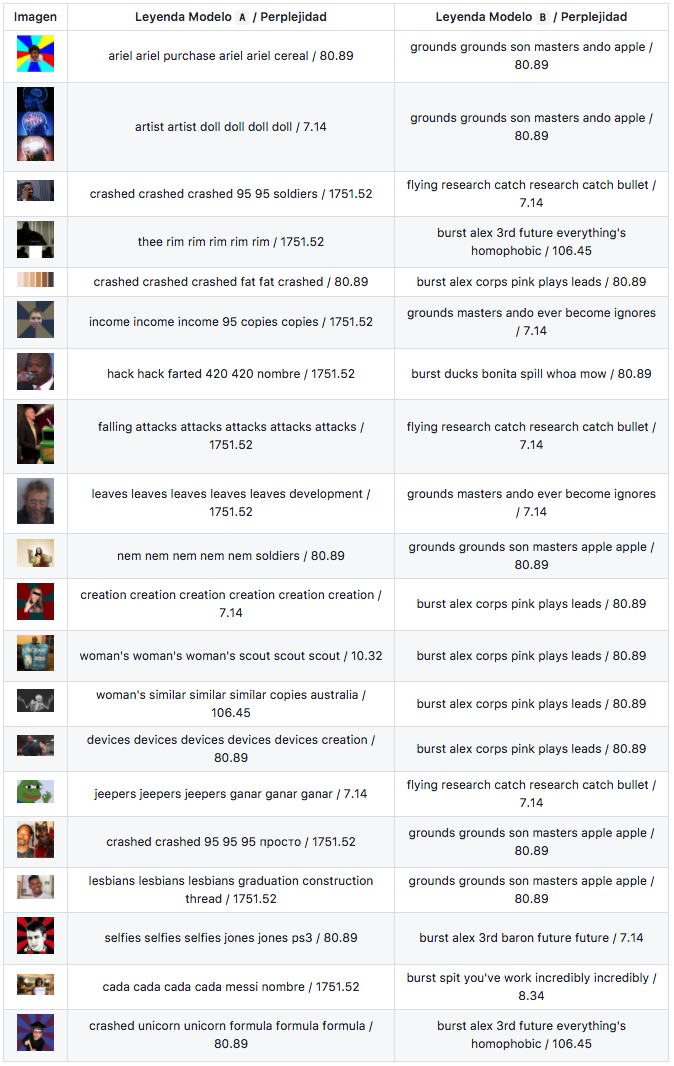
\includegraphics[width=\textwidth]{memesvsbrown}
  \caption{
    Dado un conjunto de memes nuevos, generamos leyendas para cada uno de éstos usando
    los dos mejores modelos obtenidos tras los experimentos de entrenamiento. Adicionalmente,
    para cada leyenda, calculamos la perplejidad contra el corpus \emph{Brown}.
  }
  \label{memesvsbrown}
\end{table}

\begin{table}[H]
  \centering
  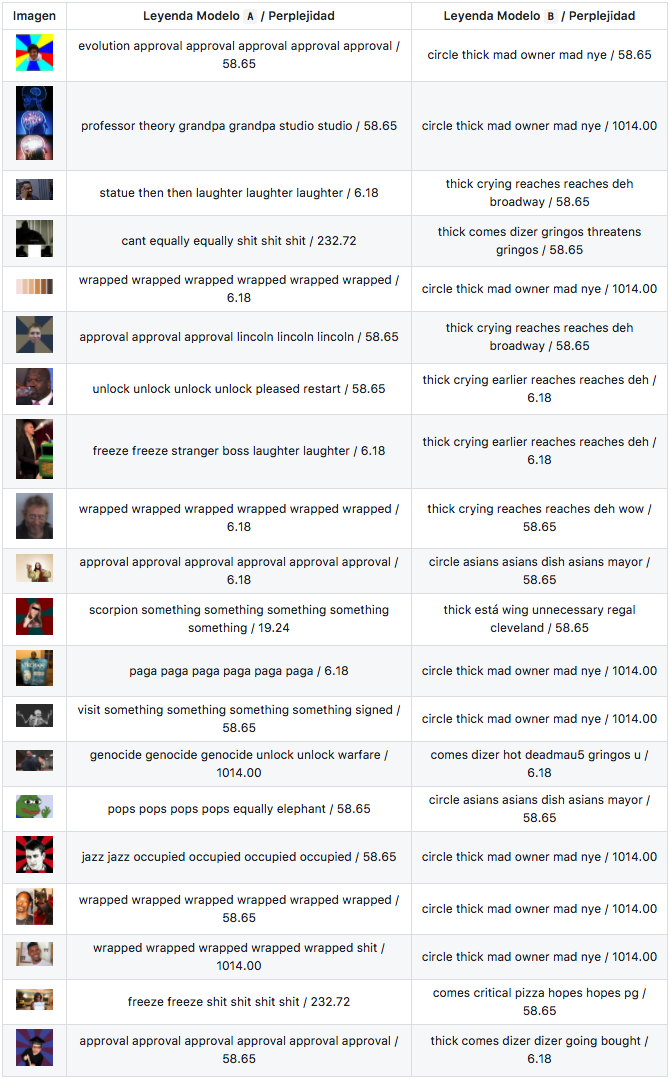
\includegraphics[width=\textwidth]{memesvsmemes}
  \caption{
    Dado un conjunto de memes nuevos, generamos leyendas para cada uno de éstos usando
    los dos mejores modelos obtenidos tras los experimentos de entrenamiento. Adicionalmente,
    para cada leyenda, calculamos la perplejidad contra el corpus obtenido de todas las leyendas\
    extraidas de internet.
  }
  \label{memesvsmemes}
\end{table}

\begin{table}[H]
  \centering
  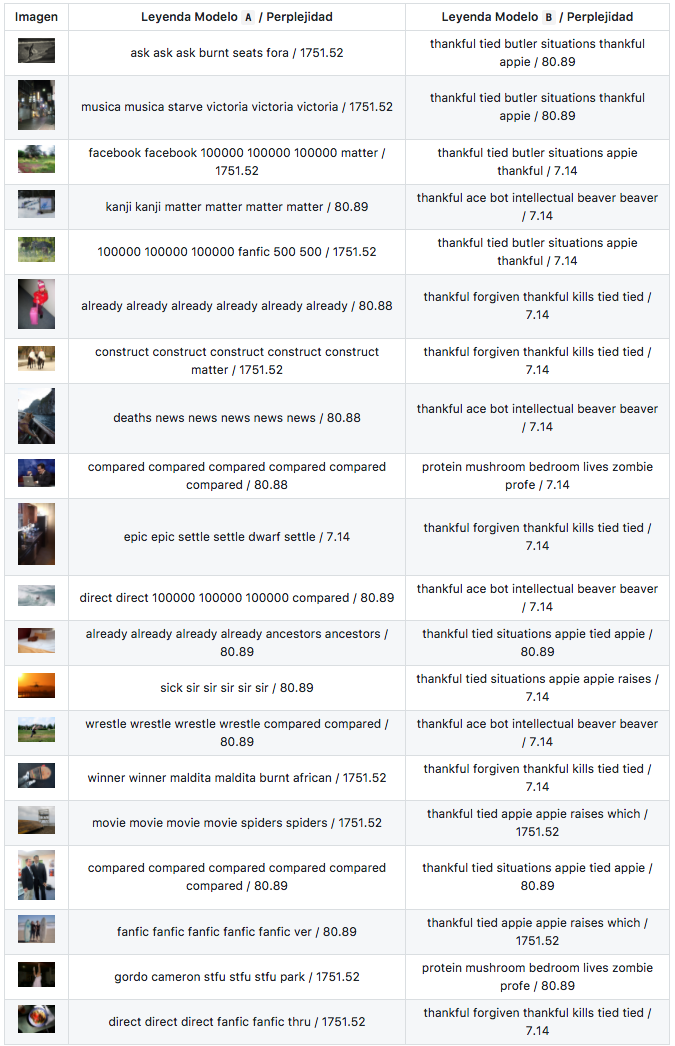
\includegraphics[width=\textwidth]{nonmemesvsbrown}
  \caption{
    Dado un conjunto de imágenes de \emph{ImageNet}, generamos leyendas para cada uno de éstos usando
    los dos mejores modelos obtenidos tras los experimentos de entrenamiento. Adicionalmente,
    para cada leyenda, calculamos la perplejidad contra el corpus \emph{Brown}.
  }
  \label{nonmemesvsbrown}
\end{table}

\begin{table}[H]
  \centering
  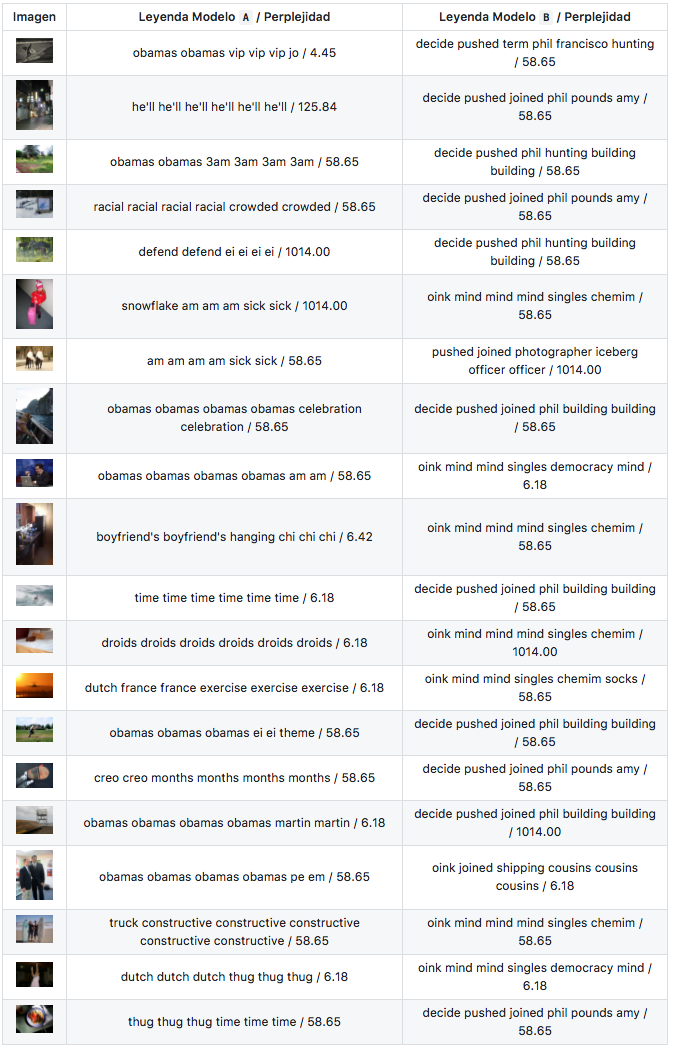
\includegraphics[width=\textwidth]{nonmemesvsmemes}
  \caption{
    Dado un conjunto de imágenes de \emph{ImageNet}, generamos leyendas para cada uno de éstos usando
    los dos mejores modelos obtenidos tras los experimentos de entrenamiento. Adicionalmente,
    para cada leyenda, calculamos la perplejidad contra el corpus obtenido de todas las leyendas\
    extraidas de internet.
  }
  \label{nonmemesvsmemes}
\end{table}


